\documentclass{article}
\usepackage{color}
\usepackage{graphicx} % Required for inserting images
\usepackage{amsmath, amssymb, amsthm} % For math symbols and environments
\usepackage{xcolor}
\usepackage{tcolorbox}
\usepackage{soul}

\newtheorem{theorem}{Theorem}
\newtcolorbox{sidework}{
  colback=gray!5!white,
  colframe=gray!75!black,
  title=Sidework
}

\usepackage{marginnote}
\usepackage{pgfplots}

\title{Math 3034 Homework}
\author{Adam Nguyen}
\date{October 2023}
\begin{document}

\maketitle

\section{Introduction}
This document contains Adam's answers to the Math 3034 homework 7.

\section{Problems and Solutions}

\subsection*{Problem 1}
Prove that there exists an \( n \in \mathbb{Z} \) such that for every \( m \in \mathbb{Z} \),
 mn + 2n + 2m + 2 = m. 

\begin{proof} 

Direct Proof

\vspace{1em}
Let n be -1 and let m be an arbitrary integer. 
Then,
\begin{equation*}
\begin{gathered}
\begin{array}{r@{{}={}}l}
mn + 2n + 2m + 2 & m(-1) + 2(-1) + 2m + 2 \\
 & -m + -2 + 2m + 2 \\
 & -m + 2m \\
& m \\
\end{array}
\end{gathered}
\end{equation*}

Thus, there exists an \( n \in \mathbb{Z} \) such that for every \( m \in \mathbb{Z} \), mn + 2n + 2m + 2 = m. 

\end{proof}
\vspace{1cm}  % Adds vertical space of 1 centimeter

\begin{sidework}

\begin{equation*}
\begin{gathered}
\begin{array}{r@{{}={}}l}
mn + 2n + 2m + 2 & m \\
mn + 2n + m + 2 & 0 \\
(mn + 2n) + (m + 2) & 0 \\
n(m + 2) + m + 2 & 0 \\
(n + 1)(m + 2) & 0 \\
\end{array}
\end{gathered}
\end{equation*}
Thus, \( n = -1 \) and \( m = -2 \) are the solutions to the equation.

\end{sidework}


\vspace{.1cm} % Adds a bit of space after your solution. Adjust as needed.


%PROBLEM2----------------------------------------------------------------------------------
\subsection*{Problem 2}

\[Let A = \{(x, y) \in \mathbb{R}^2 \mid \text{If } x = 0 \text{ then } y = 0\} \]

\vspace{.5cm} % Space between the general problem statement and the first subproblem.


%PROBLEM2a----------------------------------------------------------------------------------
\textbf{Problem 2(a):} \\
Graph the set of all elements in A on an xy-coordinate plane.
\vspace{.5cm}  % Adds vertical space of 1 centimeter

\begin{center}
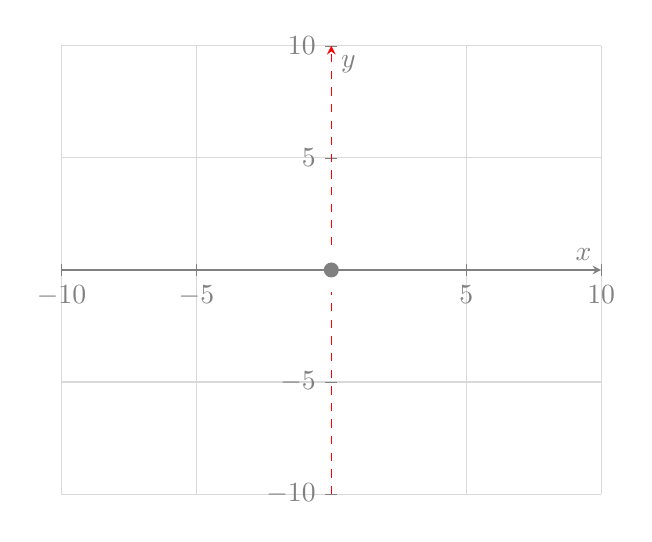
\begin{tikzpicture}
    \begin{axis}[
        axis lines = center,
        xlabel = \(x\),
        ylabel = \(y\),
        xmin = -10,
        xmax = 10,
        ymin = -10,
        ymax = 10,
        grid = both,
        grid style = {gray!30}, % Grid in gray
        x axis line style = {gray}, % x-axis in gray
        y axis line style = {red, dashed}, % y-axis in red and dashed
        xticklabel style = {color=gray},
        yticklabel style = {color=gray},
        yticklabel pos=right,
        xlabel style={gray},
        ylabel style={gray}
    ]
        % Adding the gap in the y-axis
        \addplot[white, line width=5pt] coordinates {(0,-1) (0,1)};
        % Plotting the point (0,0)
        \addplot[only marks, mark size=2.5pt, color=gray] coordinates {(0,0)};
    \end{axis}
\end{tikzpicture}
\end{center}

All points on the y-axis (marked in red) are excluded from the set of A except the origin.

\vspace{1cm} % Adjust the space as needed.




%PROBLEM2b----------------------------------------------------------------------------------
\newpage
\textbf{Problem 2(b):} \\
Prove the following statement.

For all \((x, y) \in A\), there exists an \(m \in \mathbb{R}\) such that \(y = mx\). 
\vspace{1cm}  % Adds vertical space of 1 centimeter
\begin{proof} 

Direct Proof

\vspace{1em}
Let (x, y) be an arbitrary point in A.  

\textbf{Case 1: x isn't 0}

Let m = y/x, where m is a real number. Further,
\begin{equation*}
\begin{gathered}
\begin{array}{r@{{}={}}l}
m &\frac{y}{x} \\
 m * x & \frac{y}{x} * x  \\
mx & y \\

\end{array}
\end{gathered}
\end{equation*}
\vspace{1cm}

\textbf{Case 2: x is 0}

If x is 0, then y is 0 in the set of A. Let m = 1, where m is a real number.
\begin{equation*}
\begin{gathered}
\begin{array}{r@{{}={}}l}
x & 0 \\
mx & 1 * 0 \\
    & 0 \\
    & y \\
\end{array}
\end{gathered}
\end{equation*}



Thus, for all \((x, y) \in A\), there exists an \(m \in \mathbb{R}\) such that \(y = mx\). 

\end{proof}
\vspace{1cm}  % Adds vertical space of 1 centimeter


\vspace{.5cm} % Adjust the space as needed.


%PROBLEM3a----------------------------------------------------------------------------------
\newpage
\textbf{Problem 3(a):} \\
Let \( f(x) = 2x + 4 \). Prove that for every positive real number \( \varepsilon \) there exists
a positive real number \( \delta \) such that for all \( a, b \in \mathbb{R} \), if \( |a - b| < \delta \) then
\( |f(a) - f(b)| < \varepsilon \)
\vspace{.5cm}  % Adds vertical space of 1 centimeter

\begin{proof} 

Direct Proof

\vspace{1em}
Let \( \varepsilon \) be an arbitrary positive real number more than 0 and let \( \delta \) = e/2. Suppose f(x) = 2x + 4. Let a, b be arbitrary real numbers then,
                                
\begin{align*}
    |f(a)-f(b)| &= |(2a+4)-(2b+4)| \\
                &= |2a-2b| \\
                &= 2|a-b| \\
                &<  2\delta  \\
                &=  2 (\varepsilon / 2) \\
                &= \varepsilon\\
    |f(a)-f(b)| &< \varepsilon
\end{align*}    





Thus, for every positive real number \( \varepsilon \) there exists
a positive real number \( \delta \) such that for all \( a, b \in \mathbb{R} \), if \( |a - b| < \delta \) then
\( |f(a) - f(b)| < \varepsilon \).

\end{proof}
\begin{sidework}

\begin{equation*}
\begin{gathered}
\begin{array}{r@{{}<{}}l}
|f(a)-f(b)|& \varepsilon \\
|2a+4-(2b+4)| &  \varepsilon \\
|2a-2b| & \varepsilon \\
2|a-b| & \varepsilon \\
|a-b| & \varepsilon/2 \\
\end{array}
\end{gathered}
\end{equation*}


\end{sidework}
\vspace{.25cm} % Adjust the space as needed.

%PROBLEM3b----------------------------------------------------------------------------------
\newpage
\subsection*{Problem 3(b)}
\noindent \textbf{(b)} Answer parts i. and ii. Consider the following claim:

\noindent \textit{Let \( f(x) = 2x^2 + 4 \). For every positive real number \( \varepsilon \) and for all \( a, b \in \mathbb{R} \), there exists a positive real number \( \delta \) such that if \( |a-b| < \delta \) then \( |f(a) - f(b)| < \varepsilon \).}
\vspace{.2cm}

\noindent \textbf{i.} 
The ‘proof’ provided below does not prove the given claim. Why not?

The proof below doesn't prove the given claim because there is a possibility that \( \delta \) could become undefined if \( 2|a+b| = 0\). This proof doesn't handle such a case when \( \delta \) becomes undefined.





\vspace{.5cm}
\noindent \textbf{ii.} Rewrite/modify the ‘proof’ in part i. to prove the given claim.
\begin{proof} 

Direct Proof

\vspace{1em}
Let f (x) = \(2x^2\) + 4. Let \( \varepsilon \) be an arbitrary positive real number. 

\textbf{Case 1: \( a = -b \)}


Without loss of generality, let a = -b where a and b are real numbers. Let \( \delta \) = \( \varepsilon \). Further,
\begin{align*}
    |f(a)-f(b)|&= |(2a^2+4)-(2b^2+4)| \\
 &=  |2(-b)^2-2b^2| \\
 &= |0| \\
&< \delta  \\
 &= \varepsilon \marginnote{\hspace{-3cm}\( \varepsilon \) is a real number more than 0}\\
\end{align*}

\textbf{Case 2: \( |a+b| \) isn't 0}

Let \( \delta \) = \(\frac{\varepsilon}{2|a+b|} \) and let a, b be arbitrary real numbers.  To demonstrate,

\begin{align*}
    |f(a)-f(b)|&= |(2a^2+4)-(2b^2+4)| \\
 &=  |2a^2-2b^2| \\
 &= 2|a^2-b^2| \\
 &= 2|a + b||a - b|\\
 &< 2|a + b| * \delta \\
&= 2|a + b| *  \frac{\varepsilon}{2|a+b|} \\
&= \varepsilon \\
\end{align*}
Thus, for every positive real number \( \varepsilon \) and for all \( a, b \in \mathbb{R} \), there exists a positive real number \( \delta \) such that if \( |a-b| < \delta \) then \( |f(a) - f(b)| < \varepsilon \).

\end{proof}
\begin{sidework}

\begin{equation*}
\begin{gathered}
\begin{array}{r@{{}<{}}l}
|f(a)-f(b)|& \varepsilon \\
|(2a^2+4)-(2b^2+4)| &  \varepsilon \\
|2a^2-2b^2| & \varepsilon \\
2|a^2-b^2| & \varepsilon \\
|a^2-b^2| & \varepsilon/2 \\
|a + b||a - b|& \varepsilon/2 \\
|a + b| & \frac{\varepsilon}{2|a+b|}
\end{array}
\end{gathered}
\end{equation*}
This sidework helps with understanding the original proof.

\end{sidework}
\vspace{.25cm}

\end{document}
